\chapter{System Design Overview}\label{c:sys-design}

\section{Cryostat Design}\label{sec:ch4-cryo-design}

The cryostat for the \Imager\ was designed with the goals of simplicity, reliability and turn-key automated operation.
It was built by Precision Cryogenics\footnote{Precision Cryogenics Systems, Inc. Indianapolis, IN. \url{http://www.precisioncryo.com}} to designs provided by the \Imager\ team.
The first two temperature intercept stages are provided by a Cryomech PT407 Pulse Tube Cryorefrigerator\footnote{Cryomech, Inc. Syracuse, NY. \url{http://www.cryomech.com}} (\PTC).
The PT407 has two cooling stages.
The first stage has \SI{25}{\W} of cooling power at \SI{55}{\K} while the second stage has \SI{0.7}{\W} at \SI{4.2}{\K}.
Our PT407 uses a remote motor, so that the cold head attached to the cryostat has no moving parts, minimizing vibration of the cryostat.
Vibration of the cryostat can lead to microphonic pickup either directly in the detectors themselves or in the readout circuitry, leading to much higher detector noise (see \sectionref{sec:ch6-microphonic-pickup}).

\figref{fig:cryo-cutaway} shows a cutaway view of the cryostat, and \tableref{tab:temp-optical-load} lists the temperatures typically reached by different parts of the cryostat during operation when the cryostat is open optically.
The cryostat has two main parts: a cylinder containing both the \PTC\ and the \He4-sorption refrigerator, and a box located at the bottom of the cylinder which contains temperature intercept plates and the focal plane.
There are three temperature stages: the ``\SI{80}{\K}'' Cold Plate, the ``\SI{6}{\K}'' Cold Plate, and the Focal Plane.
The \PTC\ 1st stage is connected to the \SI{80}{\K} Cold Plate by a tube of Al 1100 and a set of CDA-101 Cu braids.
The combination of this long thermal path with the high heat load on the optical filters sunk to the \SI{80}{\K} stage explains the \SI{36}{\K} temperature differential between the \SI{80}{\K} cold plate and the \PTC\ 1st stage.
The \PTC\ 2nd stage is connected to the \SI{6}{K} Cold Plate by a large (3.0 in diameter by 2.78 in long) cylinder of CDA-110 Cu\footnote{This cryostat was originally designed to work with a different cryocooler. The \PTC\ currently installed has a shorter distance between the 1st and 2nd stages; the Cu cylinder takes up this extra space.}, followed by a tube of alloy CDA-101 Cu, followed by a set of  CDA-101 copper braids.
The Cu tube is broken into two halves, and the condensation plate (see below) of the sorption fridge is clamped between these two halves.
The \SI{80}{\K} Cold Plate stands off from the cryostat vacuum jacket by four ``roll wrapped'' carbon fiber tube standoffs.
The \SI{6}{\K} Cold Plate stands off from the \SI{80}{\K} Cold Plate by eight supports made of G-10.

\begin{figure*}
\centering
\includegraphics{drawings/ch4-cryo-cutaway.pdf}
\caption[Cutaway view of the \Imager]{
  Cutaway view of the \Imager.
  \textbf{A:}\ PT407 1st stage cold head
  \textbf{B:}\ PT407 2nd stage cold head
  \textbf{C:}\ Cu cylinder connecting the PT407 2\textsuperscript{nd} stage cold head to a Cu tube, which then connects to the \He4-sorption refrigerator condensation plate.
  \textbf{D:}\ \He4-sorption refrigerator
  \textbf{E:}\ Focal Plane.
  The Cu ropes that connect the focal plane to the \SI{1}{\K} cold plate are not visible in this view.}
\label{fig:cryo-cutaway}
\end{figure*}

\begin{table*}
\centering
\caption{Temperatures Reached Under Optical Load} 
\label{tab:temp-optical-load}
\begin{tabular}{l r}
\toprule
Temperature Stage &  Temperature (K)\\
\midrule
\PTC\ 1st Stage Cold Head 			& 48 \\
\PTC\ 2st Stage Cold Head 			& 3.5 \\
Cryostat \SI{80}{\K} Cold Plate 		& 84 \\
Cryostat \SI{6}{\K} Cold Plate 			& 6.4 \\
Sorption Fridge Condensation Plate 	& 3.7 \\
Focal Plane 						& 0.970 \\
\bottomrule
\end{tabular}
\end{table*}

Options for reaching temperatures below the \abt{\SI{1.2}{\K}} transition temperature of our \TES\ detectors include: dilution refrigerators, adiabatic magnetization refrigerators, pumped \He4 baths, and \He3- and/or \He4-sorption refrigerators.
We chose a \He4-sorption fridge because the typical base temperature under no load of \abt{\SI{700}{\mK}} is well-matched to our application.
\He-sorption fridges are also inexpensive and easy to operate compared to these other solutions.
A \He4-sorption fridge works by using a charcoal adsorber to pump on a bath of liquid \He4, reducing the \He4 boiling point and thus the temperature of the bath.
The \He4 is contained within a sealed reservoir so that the refrigerator acts as a closed system requiring no \He4 replenishment. 
While \He4-sorption fridges are commercially available, our team choose to design and build a custom fridge based on a design that has been proven in astronomical applications \cite{devlin_high_2004}.

\figref{fig:he4sorp} shows a schematic depiction of the \Imager's \He4-sorption refrigerator.
The entire refrigerator is filled with \SI{2.07}{\mole} of \He4 gas, giving a pressure of \SI{900}{psi} at room temperature.
In normal operation the heat switch between the charcoal pumping chamber (``pump'') and the \He4 condensation plate is closed, keeping the charcoal close to the condensation plate temperature of \SI{3.7}{\K}, in order to adsorb as much gaseous \He4 as possible, which in turn cools the \SI{1}{\K} cold head and focal plane.

\begin{figure*}
\centering
\includegraphics{drawings/ch4-he4sorp.pdf}
\caption[Cutaway view of the \He4-sorption refrigerator]{
  Cutaway view of the \He4-sorption refrigerator.
  \textbf{A:}\ Charcoal pumping chamber (``pump'').
  The charcoal is attached to the concentric copper cylinders, used to maximize the surface area covered by the charcoal.
  \textbf{B:}\ Condensation plate.
  This copper plate is kept below the boiling point of \He4 in order to provide a point in the refrigerator for \He4 to condense and drip into the condensation pot.
  \textbf{C:}\ \He4 gas gap heat switch.
  This heat switch is used to cool the charcoal in order to pump on the \He4 bath in the condensation pot. \textbf{D:} \He4 condensation pot (``pot'').
  The condensed \He4 accumulates here.
  The concentric cylinders provide additional surface area for thermal contact to the liquid \He4.
  Not shown is a sapphire \SI{1}{\mm} constriction in the stainless steel tube connecting the pump and pot, intended to restrict the flow of super-fluid \He4 away from the pot (Swiss Jewel Company, part A34.00).
}
\label{fig:he4sorp}
\end{figure*}

Cycling the refrigerator requires four steps.
First the heat switch is opened.
The \He4-sorption refrigerator uses a \He4 gas-gap heat switch manufactured by Chase Cryogenics\footnote{Chase Research Cryogenics, Ltd. Sheffield, UK}, which requires 5 minutes of waiting time in order for the switch to fully open.
Second, the pump is heated by applying \SI{5}{\W} via a \SI{500}{\ohm} power resistor.
This power is applied until the temperature of the pump reaches 40 K, which is high enough to drive nearly all of the adsorbed \He4 off of the charcoal.
Third, the power to the pump is turned off.
Once the temperature of the condensation plate falls below the boiling point of \He4, \He4 will begin to condense on its walls, dripping into the \He4 condensation pot (``pot'').
Fourth, once the temperature of the pot has fallen to \SI{4.0}{\K}, the heat switch is turned back on.
This cools the pump, allowing \He4 to again adsorb onto the charcoal, which has the effect of pumping strongly on the pot, and cooling the \He4 contained there to the base temperature of \SI{970}{\mK} under optical load.
This process is easy to automate, and a LabVIEW program cycles the fridge automatically every night while the system is operating.

A Cryo-con Model 44\footnote{%
  Cryogenic Control Systems, Inc., Rancho Santa Fe, CA}
temperature controller is used to control the temperature of the stage, using a \SI{6.4}{\kilo\ohm} resistor attached to the focal plane.
As discussed in \sectionref{sec:ch6-common}, the temperature variations over several-minute timescales are a few parts in $10^4$ when the Cryo-con unit is used to hold the temperature steady.

Under optical load, a full cycle of the \He4-sorption refrigerator takes approximately 4 hours, reaching a base temperature of ~\SI{970}{\mK}.
When no additional load is applied the hold time is 9 hours.
When the temperature of the stage is held at the typical operating temperature of \SI{1100}{\mK} the hold time is only 3:45 hours.

\tableref{tab:fp-thermal-load} lists contributions to the heat load on the \He4-sorption refrigerator.
It excludes parasitic load inherent to the sorption refrigerator itself; we have estimated this parasitic load as \abt{\SI{0.5}{\mW}}.
% See Black n'Red notebook, Feb 3 2010.

% xxx - include data on temp vs load for the fridge?

% xxx - should really include a para explaining that the 1-K stage is
% stood-off from 4K plate by the spiders

\begin{table*}[ht]
\centering
\caption[Predicted Thermal Load on \SI{1}{\K} Stage]{
  Predicted Thermal Load on \SI{1}{\K} Stage.
  The ``Ti-6Al-4V spiders'' provide the structural link between the \SI{1}{\K} cold stage and the \SI{6}{\K} cold plate; see \sectionref{sec:ch5-focal-plane} and \figref{fig:ch5-focal-plane-back}.
  These calculations assume that the readout wiring and Ti-6Al-4V spiders are running from \SI{6.4}{\K} to \SI{1.0}{\K}.
  All wires are AWG36 Phosphor Bronze with thermal conductivity taken from the Lake Shore Cryogenics reference tables \cite{lake_shore_cryogenics_inc._cryogenic_????}.
  The load from the readout wiring is lower when running only 251 detectors because this only requires two of the five connectors carrying these wires to be connected to the focal plane.
  Assumed thermal conductivity $k$ of the Ti-6Al-4V alloy used for the spiders is $k(T) = (\SI{150}{\uW\per\cm\per\K}) T$ (William Duncan, personal communication).
  ``\BOSE\ readout wires'' refers to the wires running from room temperature used to readout the position of the secondary mirror; see \sectionref{sec:ch7-mirror-readout}.
  The heat load from these wires is high because they are not currently intercepted anywhere between room temperature and the \SI{1}{\K} stage.
  Intercepting them at the \SI{6}{\K} Cold Plate would reduce their load to \SI{1.1}{\uW}.
  ``Other optical power'' refers to in-band power that reaches the \SI{1}{\K} stage but is not absorbed by the detectors.
  The number quoted assumes that all of this power is absorbed on the \SI{1}{\K} stage; this results in an overestimate because it is likely that most of this power is reflected by the feedhorn array, rather than being absorbed.
  ``Out-of-band optical power'' is assumed to be zero because the only warm object directly illuminating the 1K stage --- the W1275 bandpass filter --- is only \SI{16}{\K}, and is not emissive at the wavelengths at which it would be radiating (see \sectionref{sec:ch4-filters} and \cite{tucker_thermal_2006}).
}
\label{tab:fp-thermal-load}
\begin{tabular}{@{}lrr@{}}
\toprule
 & \multicolumn{2}{c}{Predicted Thermal Load} \\
\cmidrule(r){2-3}
  Heat Load Source & 1004 Detectors (\si{\uW}) &  251 Detectors (\si{\uW}) \\
\midrule
  Readout wiring                   & 52 & 130 \\
  Series array \SQUID\ modules     & 0.2 & 0.6 \\ 
  % These are SA10b "two turn" according to an email from Colin. Per
  % this page: http://doc.bqemd.nist.gov/qsp/sa10b they should be
  % about 20 nW of power per chip
  \SQUID\ multiplexing chips       & 0.4 & 1.6 \\
  % Use 100 uA Ic (consistent with Colin spreadhseet) and R_dyn = 5
  % Ohms, which is guess since I don't know whether these chips are
  % low or hig R_dyn, see http://doc.bqemd.nist.gov/qsp/mux11c
  Shunt resistors                  & 5 & 18 \\
  Ti-6Al-4V spiders                & 130 & 130 \\
  Detectors (Optical + Electrical) & 0.25 & 1 \\
  Other in-band optical power      & 5.6 &   5.6 \\
  Out-of-band optical power        &   0 &   0 \\
  \BOSE\ readout wires              & 507 & 507 \\
\midrule
  Total                            & 700 & 794 \\
\bottomrule
\end{tabular}
\end{table*}

\section{Optical Design}\label{sec:ch4-optical-design}

The optical system is a Cassegrain design, chosen because circular symmetry makes these systems easy to design for on-axis performance at finite distances.
\figref{fig:ch4-optical-schematic} shows a schematic of the optical system including the focal plane.
Light enters the system from the left in this schematic, and reflects off the primary mirror onto the secondary mirror.
From the secondary mirror the light passes through a hole in the center of the primary mirror and through a window into the cryostat.
The cryostat window is a high-density polyethylene (\HDPE) lens that makes the system telecentric; this means that the focal surface of the system inside the cryostat is planar, not curved, and simplifies the design of the detector focal plane.
Smooth-walled conical feedhorns couple the incident light onto the detectors.

\begin{figure*}
\centering
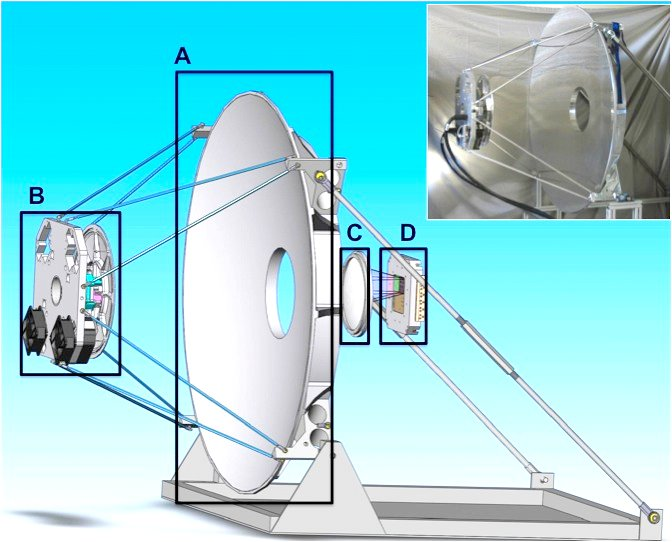
\includegraphics[width=4in]{images/optics-labeled-fixed.jpg}
\caption[Schematic showing elements of optical system]{
Schematic showing elements of optical system.
\textbf{A:} \SI{1.3}{\m} elliptical primary mirror.
\textbf{B:} Platform on which secondary mirror is mounted.
\textbf{C:} High-density-polyethylene (\HDPE) cryostat window.
           This window acts as a lens to make the system telecentric.
\textbf{D:} Detector focal plane package.
           The lid covering the focal plane holds an optical filter which defines the band of observation; see \sectionref{sec:ch4-filters}.
}
\label{fig:ch4-optical-schematic}
\end{figure*}

The secondary mirror's mount allows it to pivot and change where the system is pointing.
Two \BOSE\ linear motors\footnote{Bose ElectroForce, Framingham MA} mounted \ang{90} apart can move the mirror in arbitrary scanning patterns.
\figref{fig:ch4-optics} shows the secondary mirror mounted on its supporting platform, as well as the \BOSE\ motors.

\begin{figure*}
\centering
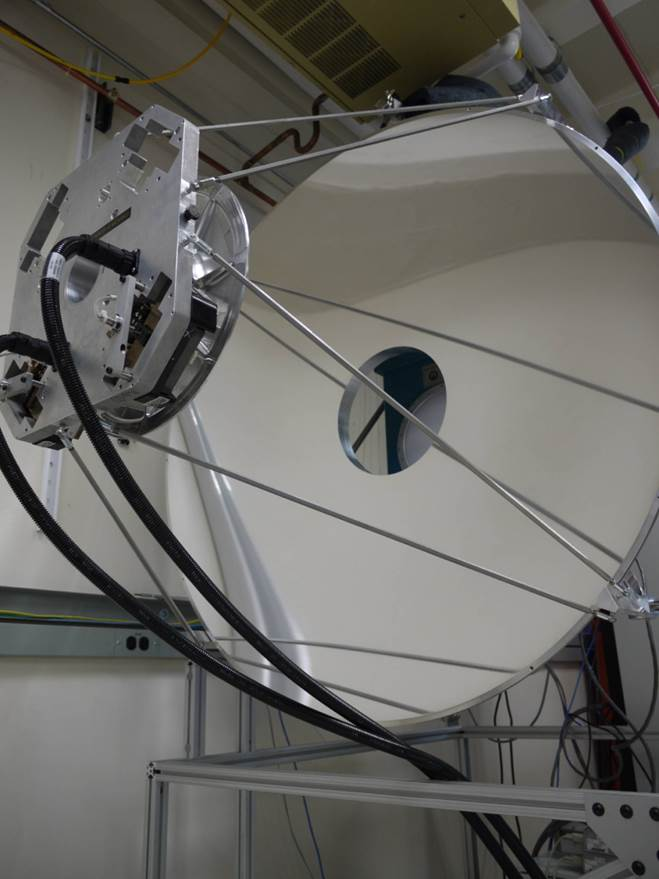
\includegraphics[width=3in]{images/optics.jpg}
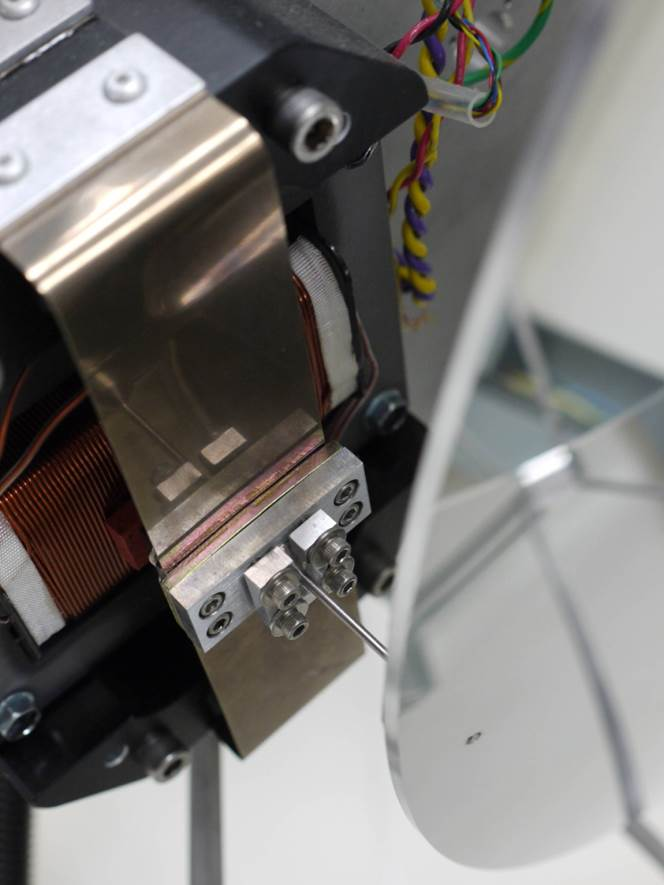
\includegraphics[width=3in]{images/optics-bose.jpg}
\caption[Photographs of the optical system]{
  Photographs of the optical system.
  \textbf{Left} The primary and secondary mirrors.
  The secondary is mounted on the Al platform in the upper left of the photograph.
  The black cables leading away from the platform go to the control system for the \BOSE\ linear motors.
  \textbf{Right} Close-up view of one of the \BOSE\ linear motors.
  The secondary mirror itself is located on the right of the photograph, while the right side of the photograph shows the \BOSE.
  A titanium strut connects the \BOSE\ to the mirror.
  % xxx would be nice to label these pictures
}
\label{fig:ch4-optics}
\end{figure*}

Scanning the secondary mirror is necessary to generate Nyquist-sampled images.
A point source in the far-field will generate an Airy intensity pattern on the focal plane with \FWHM\ $\sim 1.03 F \lambda$.
Here $F$ is the F-number of the optical system, defined as the ratio of the focal length to the aperture size.
As shown in \tableref{tab:ch4-zemax-parms}, $F = 2.0$ for the \Imager, so that the spot size on the focal plane is \abt{\SI{1.7}{\mm}}.
By the Nyquist theorem, detectors would need to be spaced every $ \SI{1.7}{\mm} / 2 \approx \SI{0.9}{\mm}$ on the focal plane to record all details of the optical image.
But the detector spacing is \SI{2.71}{\mm} (\sectionref{sec:ch4-feedhorn-design}), so that the focal plane is under-sampled by a factor of $ (2.71/0.90)^2 \approx 9$.
This problem can be overcome by scanning the system so that the ``in-between'' locations in the images are sampled. 

\tableref{tab:ch4-optical-specs} lists important properties and parameters for the optical elements of the system.
The most important parameter is the \SI{1.3}{\m} diameter of the primary mirror; this sets the resolution of the overall system.
\figref{fig:ch4-spot-diagrams} shows spot diagrams for the optical system generated by a \ZEMAX\ model for the system focused at \SI{16}{\m}.
They demonstrate that the system's optical performance is diffraction-limited over the entire focal plane for mirror rotations in both directions of up to \ang{1}, the maximum angle the mirror is displaced in operation.
\tableref{tab:ch4-zemax-parms} lists important optical properties of the system obtained from the \ZEMAX\ model.

\begin{sidewaystable}[ht]
\centering
\caption[Optical system specifications]{
  Optical system specifications.
  Some of the dimensions and parameters are listed to precisions higher than achievable manufacturing tolerances;
  these dimensions and parameters were chosen by optimization routines in \ZEMAX\, and are kept to full precision here for archival purposes.
  The shape of the elliptical and hyperbolic mirrors follows the equation $z(r) = c r^2 / (1 + \sqrt{1 - (1+k) c^2 r^2})$, where $c$ is the inverse of the mirror radius, $k$ is the conic parameter, and $r$ is the radial distance from the center of the mirrors.
  The lens surfaces follow the equation given in the table.
}
\label{tab:ch4-optical-specs}
\begin{tabular}{p{1.5in} p{1.5in} p{0.7in} p{4.5in} }
\toprule
Optical Element & Type & Outer \newline Diameter & Details \\
\midrule

Primary Mirror    & Elliptical Mirror    & \SI{1.3}{\m} 
    &  Vertex \SI{16}{\m} from far-field focal plane \\
& & &  \ZEMAX\ radius $c^{-1} = \SI{1801.453127}{\mm}$ \\
& & &  \ZEMAX\ conic $k = \num{-0.878728}$ \\
& & &  Semi-major axis: \SI{14.85}{\m} \\
& & &  Semi-minor axis: \SI{5.17}{\m} \\
& & &  Distances from mirror vertex to foci: \SI{0.93}{\m} and \SI{28.8}{\m} \\

Secondary Mirror  & Hyperbolic Mirror    & \SI{0.44}{\m}
    &  Vertex \SI{626.82}{\mm} from primary mirror vertex \\
& & &  \ZEMAX\ radius $c^{-1} = \SI{937.37187}{\mm}$ \\
& & &  \ZEMAX\ conic $k = \num{-4.466172}$ \\
& & &  Eccentricity \num{2.11} \\

Cryostat Window   & \HDPE\ Aspheric Lens & \SI{0.24}{\m}
    &  Outer vertex location depends on focus distance; see \tableref{tab:ch4-zemax-parms} \\
& & &  \SI{2}{\cm} thick at center \\
& & &  Index of refraction $n = \num{1.525}$ (\SI{7.6}{\percent} band-averaged reflection) \\
& & &  $\tan\delta = \num{4.0e-4}$ (\SI{9.1}{\percent} band-averaged absorption) \\
& & &  Outer Surface: $z(k) = c r^2 / (1 + \sqrt{1 - c^2 r^2}) + \sum_{k=1}^{k=8} \beta_k r^k$, where 
       $c^{-1} = \SI{-1052.933}{\mm}$,
       $\beta_1 = -\SI{4724.966}{\mm}$,
       $\beta_2 =  (\SI{0}{\mm})^{-2}$,
       $\beta_3 =  (\SI{88.649}{\mm})^{-3}$,
       $\beta_4 = -(\SI{67.854}{\mm})^{-4}$,
       $\beta_5 =  (\SI{90.995}{\mm})^{-5}$,
       $\beta_6 =  (\SI{89.966}{\mm})^{-6}$,
       $\beta_7 = -(\SI{97.618}{\mm})^{-7}$,
       $\beta_8 = -(\SI{191.31}{\mm})^{-8}$ \\
& & &  Inner Surface: $z(k) = c r^2 / (1 + \sqrt{1 - c^2 r^2}) + \sum_{k=1}^{k=8} \beta_k r^k$, where 
       $c^{-1} = \SI{-699.782}{\mm}$,
       $\beta_1 = -\SI{62.359}{\mm}$,
       $\beta_2 =  (\SI{0}{\mm})^{-2}$,
       $\beta_3 = -(\SI{45.520}{\mm})^{-3}$,
       $\beta_4 =  (\SI{59.477}{\mm})^{-4}$,
       $\beta_5 = -(\SI{74.141}{\mm})^{-5}$,
       $\beta_6 =  (\SI{86.306}{\mm})^{-6}$,
       $\beta_7 = -(\SI{107.763}{\mm})^{-7}$,
       $\beta_8 = -(\SI{124.984}{\mm})^{-8}$ \\
Detector Focal Plane &                   & N/A           &  \SI{171.541}{\mm} from vertex of inner surface of cryostat window \\
\bottomrule
\end{tabular}
\end{sidewaystable}

% Here is how I calculated the inner/outer marginal rays using
% ZEMAX. It is a bit of a pain.
% 
% Click on "Gen" for the "General" dialog. Go to the "Aperture
% Tab". Under "Aperture Type" choose "Object Cone Angle". This sets
% the angle of the outermost ray. Now you can keep trying different
% angles and looking at the ray layout (Lay or L3d) until you find the
% ray that is touching the very edge of the secondary. Do this for
% both the outer and inner case --- secondary limits *both* cases, just
% in different ways!
%
% To get the offset (x) distance on the primary mirror, zoom in on
% where that ray crosses the primary and find the offset by looking
% at the coordinates in the title bar.
%
% The results are:
% 
% 16 m
% 
% inner - 5.142 deg / 229.10569 mm on primary
% outer - 13.61 deg / 610.40411
% 
% 17 m
% 
% inner - 5.252 deg / 228.59374 mm on primary
% outer - 14.025 deg / 614.50288 on primary
% 
% 28 m
% 
% inner - 5.989 deg / 225.12397 mm on primary
% outer - 16.908 deg / 642.22731 mm on primary

\begin{sidewaystable}[ht]
\centering
\caption[Parameters of the optical system extracted from \ZEMAX\ simulations]{
  Parameters of the optical system extracted from \ZEMAX\ simulations.
  ``Focus Distance'' is the distance from the vertex of the primary mirror to the far-field plane at which the system is focused.
  ``Lens Distance'' is the distance from the outer vertex of the lens to the vertex of the primary.
  ``Plate Scale'' gives the ratio of distances on the far-field focal plane to the detector focal plane.
  ``Mirror Rotation'' gives the distance that the on-axis point moves when the mirror is rotated by \ang{1}.
  ``F-Number'' gives the ratio of the focal distance to the aperture size as viewed from the detector focal plane; this the ``Working F/\#'' from \ZEMAX.
  ``Marginal Rays'' gives the angle away from the optical axis of the inner/outer marginal rays; these are the most extreme rays emerging from the detector focal plane that reach the far-field focal plane.
  ``Primary Range'' gives the innermost and outermost radius of the primary that is actually used, e.g., when focused at \SI{16}{\m}, the outer \SI{4}{\cm} of the primary is not used.
}
\label{tab:ch4-zemax-parms}
\begin{tabular}{ccccccc}
\toprule
  \specialcell{Focus Distance \\ (\si{\m})} &
  \specialcell{Lens Distance \\ (\si{\mm})} &
  \specialcell{Plate Scale \\ (\si{\cm}/\si{\cm})} &
  \specialcell{Mirror Rotation \\ (\si{\cm}/\si{\degree})} &
  \specialcell{F-Number  \\ } & 
  \specialcell{Marginal Rays \\ (\si{\degree})} &
  \specialcell{Primary Range \\ (\si{\mm})} \\
\midrule
16 & 230.475 &  6.111 & 18.354 & 2.01 &  \ang{5.14} / \ang{13.61} & 229.1 / 610.4 \\
17 & 197.18  &  6.638 & 19.330 & 1.96 &  \ang{5.24} / \ang{14.03} & 228.6 / 614.5 \\ 
28 &   8.0   & 12.589 & 30.037 & 1.71 &  \ang{5.99} / \ang{16.91} & 225.1 / 642.2 \\
\bottomrule
\end{tabular}
\end{sidewaystable}

\begin{figure*}
\centering
\begin{tabular}{lr}
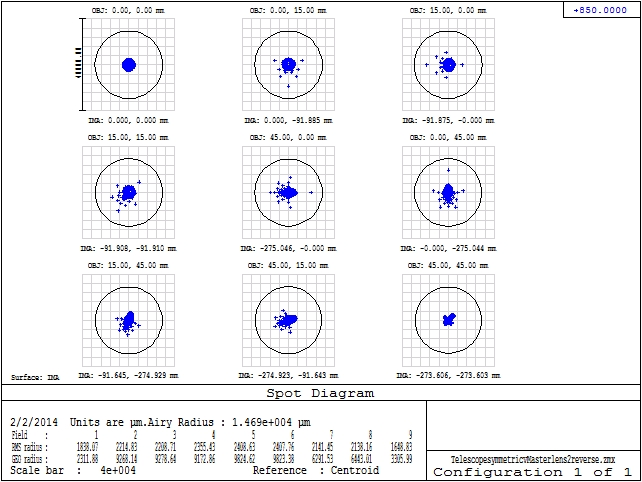
\includegraphics[width=3in]{images/ch4-zemax-spot-0-0.JPG}
 &
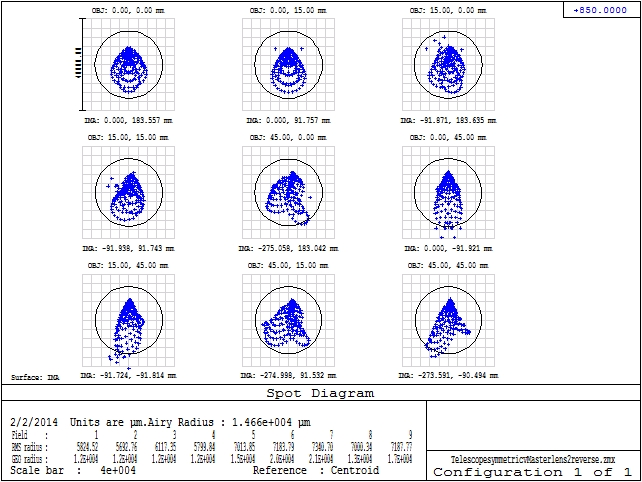
\includegraphics[width=3in]{images/ch4-zemax-spot-1-0.JPG}
 \\
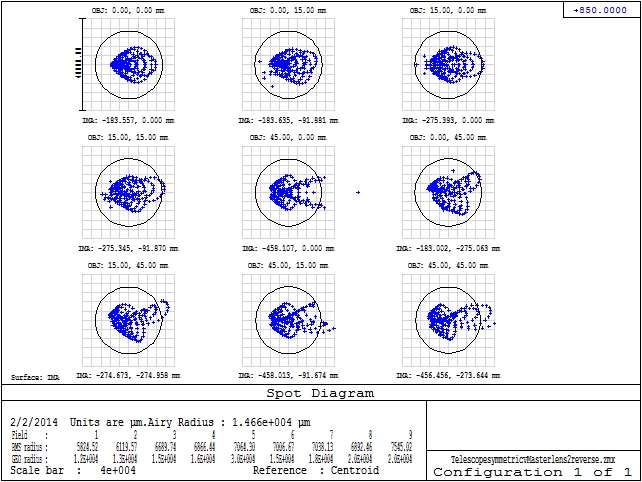
\includegraphics[width=3in]{images/ch4-zemax-spot-0-1.JPG}
 &
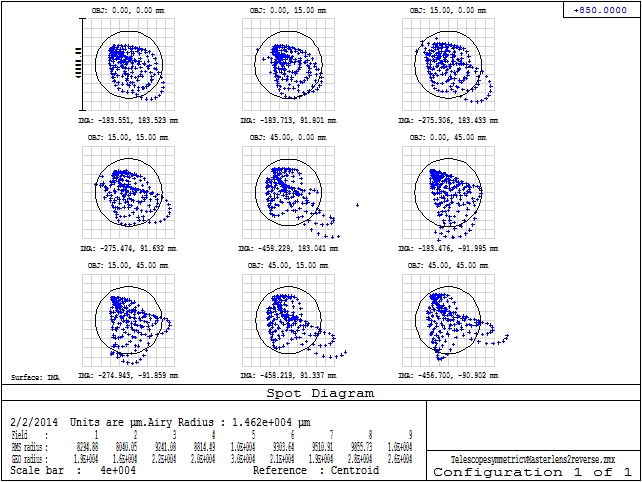
\includegraphics[width=3in]{images/ch4-zemax-spot-1-1.JPG}
\end{tabular}
\caption[\ZEMAX\ spot diagrams]{
\ZEMAX\ spot diagrams for the \Imager's optical system when focused to \SI{16}{\m}.
This represents the distribution of points on the focal plane to which rays from a point on the object trace to.
Each plot shows spot diagrams for nine points in the focal plane covering the area over which detectors in the sub-array are located.
The four plots (moving left to right and top to bottom) are for the secondary mirror with no tilt, \ang{1} tilt about one axis, \ang{1} title about other axis, and \ang{1} tilt about both axes.
The black circle gives \ZEMAX's estimate of the size of the Airy disk for the optical system, which is defined as the location of the first null in the system's diffraction pattern.
In all cases, nearly all rays map to within the Airy disk, indicating that the performance of the optical system is diffraction-limited.
}
\label{fig:ch4-spot-diagrams}
\end{figure*}

The \HDPE\ window does not have an anti-reflection coating.
The index of refraction of \HDPE\ is $n=1.525$ with an absorption coefficient at \SI{350}{\GHz} of $\alpha = \SI{0.044}{\cm^{-1}}$ \cite{lamb_miscellaneous_1996}.
Using the standard formulas for Fabry-Perot fringing when light passes through a lossy \SI{2}{\cm} thick dielectric slab \cite[Chapter~5]{sophocles_j._ordanidis_electromagnetic_2014}, the band-averaged transmission through the window is calculated to be \SI{84}{\percent}, with \SI{7.6}{\percent} reflection due to the change in dielectric constant, and \SI{9.1}{\percent} due to absorptive loss in the dielectric.

\section{Optical Filtering} \label{sec:ch4-filters}

A series of optical filters located inside the cryostat serves to reduce the thermal load on the \SI{1}{\K} focal plane and to define the observing band.
These filters are shown schematically in \figref{fig:ch4-filter-stack}.
These filters include thin thermal blocking filters located at \SI{300}{\K}, \SI{80}{\K}, and \SI{6}{\K}; multi-layer lowpass filters at \SI{80}{\K} and \SI{6}{\K}; and a band-defining filter located at \SI{1}{\K}.
The transmission properties of these filter listed in this section are from measurements made at Cardiff University, where the filters were made.

\begin{figure*}
\centering
\includegraphics{drawings/ch4-filter-stack.pdf}
\caption[Schematic showing locations of all filters in the \Imager]{
  Schematic showing locations of all filters in the \Imager.
  Everything shown here is internal to the cryostat.
  On the left the nominal temperatures for each stage are listed, and on the right the names and cutoff wavelengths are listed.
}
\label{fig:ch4-filter-stack}
\end{figure*}

The transmission of the bandpass filter is plotted in blue in \figref{fig:ch4-bandpass}.
The integrated bandwidth of the bandpass filter is \SI{31.1}{\GHz}, with a full-width-half-maximum (\FWHM) band of \SI{35.0}{\GHz}.
There is some ambiguity in defining the bandwidth and efficiency of a bandpass filter that does not have a top-hat shape.
In this thesis I have chosen to described the filter as having a bandwidth of \SI{35.0}{\GHz} with efficiency $31.1 / 35.0 = \SI{88.5}{\percent}$.

\begin{figure*}
\centering
\includegraphics{./drawings/ch4-bandpass.pdf}
\caption[Plot showing transmission of the bandpass filter.]{
  Plot showing transmission of the bandpass filter.
}
\label{fig:ch4-bandpass}
\end{figure*}

The thermal blocking filters are sheets of \SI{3.3}{\um} polypropylene with capacitive metal grids printed on each side.
Because they are so thin, these filters have little emission even at the infrared wavelengths at which polypropylene is highly absorptive \cite{tucker_thermal_2006}.
The cutoff wavelengths of these filters are listed in \tableref{tab:ch4-filter-stack}.

The \Imager\ also contains thicker multi-layer filters that act as lowpass filters at wavelengths closer to the observing band.
These filters are also made of metal meshes and polypropylene, but many meshes and polypropylene layers are sandwiched together to form filters that are \abt{\SI{1}{\mm}} thick.
These filters have excellent transmission in-band as well as good out-of-band rejection \cite{ade_review_2006}, but the thick polypropylene substrates mean that they are also highly absorptive --- and thus also emissive -- in the near-infrared.
Additionally, polypropylene has poor thermal conductivity.
This means that unless they are heat-sunk very well, the centers of the filters will be much warmer than the stage at which they are anchored, and so they will re-radiate infrared power into the cryostat.
The filters in the \Imager\ are clamped in place using spiral springs, using a design that is similar to that used by the Atacama Cosmology Telescope receiver \cite{swetz_overview_2011}.

\tableref{tab:ch4-filter-stack} lists all filters in the system and gives temperatures for the centers of some of the filters, taken while the cryostat was open optically.
The outermost multi-layer filter is very warm (\SI{190}{\K}), and this is a significant source of loading on the \SI{6}{\K} stage, which also warms the \SI{6}{\K} multi-layer filters, leading to a level of loading on the \SI{1}{\K} stage that prevents it from being cooled below \SI{1.2}{\K} unless the aperture is stopped down to reduce IR loading.
This has been accomplished with a \SI{2.875}{\in} by \SI{2.875}{\in} aperture installed between the thermal blocking and multi-layer filters on the \SI{80}{\K} stage.
With this aperture installed, the bandpass filter center reaches a temperature of \SIrange{4}{8}{\K} (varying based on the size of the aperture stop).

\tableref{tab:ch4-filter-stack} also lists the in-band transmission of each filter.
The total transmission of the filter stack excluding the bandpass filter is \SI{88.4}{\percent}.

\begin{table*}
\centering
\caption[Details of all filters installed in the \Imager]{
  Details of filters installed in the \Imager.
  The filters are listed in order from the outside of the cryostat to the inside.
  ``Stage'' refers to the cryostat temperature stage at which the filter is located.
  ``Cutoff'' refers to the point at which the filter transmission falls to \abt{-10}\,dB.
  ``Transmission'' gives the band-averaged transmission of the filter.
  ``Temperature'' gives the temperature at the center of a filter as measured by embedding a diode in a blob of Apiezon-N thermal grease placed on top of a layer of Kapton tape (which prevents applying grease to the filter itself).
  The temperature of W1428 was measured without the aperture stop in place and while it was located after THERM3 rather than before.
  The current placement of this filter between two thermal blocking filters prevents measuring its temperature in the current configuration.
  The temperatures for W1269 and W1275 were measured both with and without a $(\SI{2.25}{\in})^2$ aperture stop, which covers \SI{40}{\percent} less area than the stop used in all other measurements in this thesis.
 Temperature measurements are not available for the other filters. 
}
\label{tab:ch4-filter-stack}
\begin{tabular}{llcccc}
\toprule
  \specialcell{Stage} &
  \specialcell{Filter Label} &
  \specialcell{Cutoff \\ (\si{\um}) } &
  \specialcell{Cutoff \\ (\si{\THz}) } &
  \specialcell{Transmission} & 
  \specialcell{Temperature \\ (\si{\K})} \\
\midrule
\SI{300}{\K} & THERM1 \SI{1.9}{\um}    & 1.9 & 158  & 1.00   &     \\
\SI{80}{\K} & THERM2 \SI{4}{\um}      & 4   & 75   & 1.00   &     \\
            & W1428 \SI{18}{\cm^{-1}} & 556 & 0.54 & 0.96   & 193 \\ % cooldown 12 6/9/10
            & THERM3 \SI{6}{\um}      & 6   & 50   & 1.00   &     \\
\SI{6}{\K}  & THERM4                  &     &      & 1.00   &     \\
            & W1266 \SI{14}{\cm^{-1}} & 714 & 0.42 & 0.94   &     \\
            & W1269 \SI{32}{\cm^{-1}} & 313 & 0.96 & 0.98   & 14--37   \\ % cooldowns 30 & 31
\SI{1}{\K}  & W1275                   & N/A & N/A  & 0.885 & 3.7--7.8 \\ % cooldowns 30 & 31
\bottomrule
\end{tabular}
\end{table*}

% is ripple in FTS results at low frew for lowpass filters due to
% reflection from the polypropylene?

\section{Feedhorn Design}\label{sec:ch4-feedhorn-design}

Millimeter and submillimeter astronomical instruments using \TES\ detectors use many different strategies for coupling light onto detectors, including filled arrays of absorbers \cite{swetz_overview_2011,holland_scuba-2:_2013}, antennas with lenslets \cite{keating_ultra_2011}, phased antenna arrays \cite{obrient_antenna-coupled_2012}, corrugated feedhorns \cite{austermann_sptpol:_2012,niemack_actpol:_2010}, and smooth-walled conical feedhorns \cite{schwan_invited_2011,carlstrom_10_2011}.
The \Imager\ uses smooth-walled conical feedhorns because they are easy to design and easy to machine.
Smooth-walled feedhorns do not have the low cross-polarization properties of corrugated feedhorns \cite{clarricoats_corrugated_1984}, but this is not a concern here because the \Imager's detectors are polarization-insensitive.

Although the \Imager\ is always receiving radiation, never transmitting, this thesis often refers to the transmitting beam pattern, because in some cases this is easier to conceptualize.
Beams in transmission and reception are the same, a consequences of the reciprocity relationships obeyed by the Maxwell equations(see, e.g.\ \cite{balanis_antenna_2005}).

\figref{fig:feedhorn-parms} depicts a smooth-walled conical feedhorn and its interaction with the optical system.
Although the optical system has a secondary mirror as well, for the purposes of feedhorn design an equivalent optical system with only one mirror can be used, with the same focal length \cite{goldsmith_quasioptical_1998}.

If a feedhorn is observing a temperature distribution $T_{target}(\theta,\phi)$, and is pointed in a direction $(\theta_0, \phi_0)$, then the temperature observed by the feedhorn will be
\begin{equation}
    T_{eff}(\theta_0,\phi_0) = \int \, d \Omega \, T_{target}(\theta - \theta_0,\phi - \phi_0) P(\theta,\phi).
\end{equation}
The function $P$ is called the ``beam'' or ``beam pattern'' of the feedhorn, and describes the angular pattern of radiation to which the feedhorn is sensitive.
When using this expression one must keep in mind that the fraction of the beam that spills off the primary mirror (e.g.\ the unshaded region in \figref{fig:feedhorn-parms}) will see not the temperature distribution of the target, but a temperature distribution determined by what is beyond the primary mirror\footnote{Because of the presence of the secondary mirror, some of this temperature distribution will be in front of the system, and some will be behind.}.
The fraction of the beam that strikes the primary mirror and proceeds to the target is called the spillover efficiency $\eta_s$.

\begin{figure*}
\centering
\includegraphics{drawings/ch4-feedhorn-parms.pdf}
\caption[Schematic showing important parameters of a feedhorn and its beam]{
  Schematic showing important parameters of a feedhorn and its beam.
  The beam appears to emerge from the phase center, a distance $l_c$ behind the mouth of the feedhorn in this diagram.
  The main lobe of the beam is approximated well by a Gaussian, here characterized by a full-width-half-maximum (\FWHM) beam width.
  The shaded fraction of the Gaussian represents the part of the beam that falls onto the primary mirror and reaches the target.
  As discussed in the text, for the purposes of feedhorn design the secondary mirror can be ignored and the system treated as a system of feedhorns illuminating only a primary mirror with a hole in its center.}
\label{fig:feedhorn-parms}
\end{figure*}

The important design parameters for a smooth-walled conical feedhorn are the opening diameter $D$ and the opening half-angle $\alpha_0$.
The feedhorn opening diameter $D$ is chosen to minimize the total \NETD\ of the system.
The total \NETD\ was given in \sectionref{sec:ch1-netd-reqs} as
\begin{equation}
    NETD = \frac{NEP_{tot}}{2 k_B \Delta \nu \eta_{tot} \sqrt{2 \tau}}.
\end{equation}
To make the factors depending on the size of the feedhorns more clear we can break the optical efficiency $\eta_{tot}$ into a product of two factors, $\eta_s$ and $\eta_{other} = \eta_{tot} / \eta_s$.
We then note that the integration time per pixel $\tau$ is proportional to the number of detectors $N$.
This leads to
\begin{equation}
    NETD \propto \frac{NEP_{tot}}{\sqrt{N}\eta_s}.
\end{equation}

The critical relationship is that as a feedhorn's opening diameter increases, the width of the beam becomes smaller.
Small beam angles increase $\eta_s$, which improves \NETD.
However, the diffraction-limited area on the focal plane that can be covered by feedhorns is fixed, so that increases in the horn opening diameter reduce the number of detectors $N$, which worsens \NETD.
Choosing an optimal feedhorn size requires trading these two effects off against each other to minimize \NETD.

There are four additional factors to consider.
First, $NEP_{tot}$ is not independent of $\eta_s$.
In a system that is photon-noise-limited, $NEP_{tot}$ may worsen, stay the same, or improve, depending on the temperature seen by the spilled over portion of the beam.
Indoors, all of the beam will see roughly the same temperature as the target, so that total photon noise will stay the same.
Outdoors the situation is more complicated because the temperature seen by the spilled over beam will depend on the local scenery and weather conditions.
For simplicity, the analysis of optimum feedhorn size in this chapter makes the assumption that the noise seen by a detector is independent of the beam size.

Second, for a Cassegrain optical system, $\eta_s$ is not a monotonic function of $D$, because the secondary mirror obstructs the central part of the beam, preventing it from reaching the target.
This means that narrow beams can have poor $\eta_s$ because a large fraction of the main lobe of the beam will be blocked.

Third, the dependence of the number of detectors $N$ on the feedhorn diameter $D$ is not a smooth function, because it is not possible to have, e.g., 1/3 of a feedhorn.
As explained in \sectionref{sec:ch5-layout}, the \Imager's detectors are laid out on a square grid.
So it is more helpful to think of the feedhorn diameter as taking on a discrete set of values that depends on the number of feedhorns per each side of the grid.

Finally, the choice of readout system and wiring places a firm upper limit of \num{1024} on the number of detectors in the system.

A \MATLAB\ program was used to find the optimum feedhorn size.
The program uses an analytic expression for the beam pattern developed in \cite{green_radiation_2006,narasimhan_modes_1971,}.
The far-field electric field pattern takes the form
\begin{equation}
    \vect{E}(\theta,\phi) = E_{\theta}(\theta) \sin{\phi} \hat{\theta} + E_{\phi}(\theta) \cos{\phi} \hat{\phi}.
\end{equation}
Here $E_{\theta}$ and $E_{\phi}$ are functions depending the horn diameter $D$ and opening half-angle $\alpha_0$, and involving definite integrals of Bessel functions, given in \cite{green_radiation_2006,narasimhan_modes_1971}.
This expression is for the waveguide mode polarized along the $\pi/2$ direction.
The \Imager's detectors are unpolarized, so they detect both waveguide polarizations equally; see \sectionref{sec:ch4-coupling} for confirmation of this via simulations.
The total power beam map is thus given by the incoherent sum
\begin{equation}
    P(\theta, \phi) = |\vect{E}(\theta, \phi)|^2 + |\vect{E}(\theta, \phi+\pi/2)|^2,
\end{equation}
which simplifies to 
\begin{equation}
    P(\theta) = |E_{\theta}(\theta)|^2 + |E_{\phi}(\theta)|^2,
\end{equation}
which is independent of $\phi$, as expected for an unpolarized detector.

To calculate the spillover efficiency of an individual feedhorn, the \MATLAB\ program integrates $P$ over the angles $\theta$ that illuminate the primary mirror and reach the target: \SIrange{5.2}{14.0}{\degree} at \SI{17}{\m}\footnote{see \sectionref{sec:ch4-optical-design}}.
\figref{fig:ch4-feed-spill} shows a contour plot of spillover efficiency for an individual conical feedhorn as a function of $D$ and $\alpha_0$.
The black dot shows the parameters for the feedhorns chosen for the \Imager.
This plot shows that $\eta_s$ depends much more strongly on $D$ than on $\alpha_0$.
$\alpha_0 = \SI{9.4}{\degree}$ was chosen as a value that is easy to machine, keeps the thermal mass of the feedhorn array low (small values of $\alpha_0$ lead to long feedhorns and higher thermal mass), and is not too far from the maximum achievable $\eta_s$ for any fixed feedhorn diameter $D$.

\begin{figure*}
\centering
\includegraphics{./drawings/ch4-feed-spill.pdf}
\caption[Feedhorn spillover efficiency]{
  Plot showing feedhorn spillover efficiency $\eta_s$ as a function of horn diameter $D$ and horn flare half-angle $\alpha_0$.
  The blue dotted line is for $\alpha_0 = \ang{9.4}$, the value assumed during optimization.
  The black dot shows the feedhorn parameters used in the \Imager: $D = \SI{2.68}{\mm}$ (cold) and $\alpha_0 = \ang{9.4}$
}
\label{fig:ch4-feed-spill}
\end{figure*}

To find the number of horns per array size that minimizes \NETD\, the program assumes that the feedhorns must cover a square \SI{43.9}{\mm} per side.
It allows for \SI{1}{\mil} spacing between the edges of the feedhorns, and also accounts for a thermal contraction factor of 4.14 parts per thousand \cite[Appendix~A6.4]{ekin_experimental_2006}.
Four horns from each sub-array are assumed to be missing in order to accommodate other features on the detector wafer.
The resulting \NETD\ estimates --- normalized to the \NETD\ for the actual feedhorns chosen --- is shown in \figref{fig:ch4-netd-vs-nfeeds}.
The optimal number of feedhorns per array side is 19, for a total (across all four sub-arrays) of 1428 feedhorns of diameter \SI{2.25}{\mm} cold.
Because of readout limitations, the actual number of detectors per side is 16, for 1004 feedhorns with diameter \SI{2.68}{\mm} (\SI{108}{\mils} at room temperature)\footnote{%
Five locations in the $16 \times 16$ grid are missing detectors; see \sectionref{sec:ch5-layout}.}.
The loss in \NETD\ from this sub-optimal choice is only \SI{1.7}{\percent}.

\begin{figure*}
\centering
\includegraphics{./drawings/ch4-netd-vs-nfeeds.pdf}
\caption[\NETD\ vs number of detectors]{
  Plot showing how \NETD\ depends on the number of feedhorns in each sub-array.
  As discussed in the text, due to the square array the important parameter determining the total number of feedhorns is the number per side of the grid.
  The \NETD\ is plotted relative to the \NETD\ for an array with 16 feedhorns per side, which is the value chosen for this system.
  \NETD\ is minimized with 19 feedhorns per side, giving a total of 1428 feedhorns of diameter \SI{2.25}{\mm} (cold), but the \Imager\ uses 1004 feedhorns of diameter \SI{2.68}{\mm} (cold) because of readout limitations.
  The cost in \NETD\ is only \SI{1.7}{\percent}.
}
\label{fig:ch4-netd-vs-nfeeds}
\end{figure*}

% xxx - need to re-run all data analysis after verifying the proper
% inner angle!!!!

\figref{fig:ch4-beams} contains plots of both the beam pattern for the conical feedhorn and the far-field beam pattern of the entire optical system (also called the ``point spread function'').
The feedhorn beam pattern follows the model described above.
The far-field beam pattern accounts for the fact that the beam is truncated by the secondary mirror in its center and by the edge of the primary at its edge; these limits are plotted as vertical blue lines on the left plot.
The truncation of the center of the beam is responsible for the side-lobe of magnitude \abt{\SI{5.7}{\percent}} that is visible in the far-field beam pattern.
The far-field beam has a \FWHM\ of \SI{1.38}{\cm} for a point source.
After convolution with a \SI{0.2}{\in} circle the \FWHM\ is \SI{1.39}{\cm}, and after convolving with a \SI{1.791}{\cm} circle (same size as a dime) the \FWHM\ is \SI{1.76}{\cm}.

\begin{figure*}
\centering
\includegraphics{./drawings/ch4-beams.pdf}
\caption[Beam patterns]{
  Plots showing theoretical beam pattern for the design feedhorns.
  \textbf{Left} The unpolarized power pattern for a conical feedhorn with diameter \SI{2.68}{\mm} and opening half-angle $\alpha_0 = \ang{9.4}$, at the center frequency for our band.
  The region between the vertical blue lines indicates the part of the beam that strikes the primary mirror and reaches the far-field focal plane.
  Also plotted is the best-fit Gaussian within the blue lines.
  The \FWHM\ beam width is \ang{10.6}.
  \textbf{Right} \SI{17}{\m} theoretical far-field unpolarized power pattern.
  The plot includes the effect of blockage by the secondary mirror as well as the edge taper of the beam on the primary.
  The \FWHM\ beam width is \SI{1.38}{\cm}.
  The side-lobe is caused by the secondary mirror, and is \SI{5.7}{\percent} high.
}
\label{fig:ch4-beams}
\end{figure*}

The feedhorns were machined out of Al 6061 and then Au-plated.
An estimate of the insertion loss of the feedhorns requires the conductivity of this plated Au at \SI{1}{\K}, but this quantity is not known.
I assumed that the Au has the standard value for conductivity at room temperature of \SI{41e6}{S\per\m}, with a residual resistivity ratio of 3.
Using this value, and assuming a surface roughness of \SI{5}{\um}, \HFSS\ simulations predict an insertion loss of \SI{-10.5}{\dB}, including both the feedhorn and the waveguide.
This corresponds to a feedhorn efficiency of \SI{91}{\percent}.
\HFSS\ simulations indicate that the return loss for the feedhorns is \SI{-28}{\dB}, so I ignore return loss.

\section{Optical Coupling to Detectors} \label{sec:ch4-coupling}

The feedhorns described in \sectionref{sec:ch4-feedhorn-design} couple incoming light into circular waveguide.
The waveguide carries the light to the bolometer, where it is absorbed by a Palladium Gold (PdAu) mesh.
This section describes the waveguide and absorbing structures.

The diameter of the circular waveguide was chosen to place the cutoff frequency of the first propagating mode (TE11) below the optical band of the \Imager.
The cutoff frequency of this mode is given by \cite[Chapter~5]{harrington_time-harmonic_2001}:
\begin{equation} \label{eqn:ch4-te11-cutoff}
  f_c = \frac{1.841 c}{2 \pi a },
\end{equation}
where $c$ is the speed of light in free space and $a$ is the radius of the waveguide.
For our waveguide I chose a diameter of \SI{0.6}{\mm}, which gives a cutoff frequency of \SI{292}{\GHz}, well below the lowest frequency in the band.
This choice was made so that the waveguide impedance was more uniform across the waveguide, which makes designing an efficient absorbing structure easier.

The ideal absorbing structure for unpolarized light would be to cover the entire area of the waveguide with a sheet having a surface impedance equal to the waveguide impedance.
The characteristic impedance at frequency $f$ for a TE mode in waveguide is \cite[Chapter~2]{harrington_time-harmonic_2001}
\begin{equation} \label{eqn:ch4-wg-imp}
  Z (f) = \frac{\eta_f}{\sqrt{1 - (f_c/f)^2}}\,,
\end{equation}
where $\eta_f \approx \SI{377}{\ohm}$ is the impedance of free space and $f_c$ the cutoff frequency for the mode.
For our waveguide, the impedance at the band-center frequency of \SI{347}{\GHz} is \SI{700}{\ohm}.
The highest-resistance material available in the fabrication process for the \Imager's detectors is a \SI{20}{\nm} thick layer of PdAu, which for our fabrication process has a surface impedance of \SI{12}{\ohm}/sq, far too low to serve as an effective full-width waveguide absorber.

However, the \SI{12}{\ohm}/sq PdAu can still be used to create an absorbing structure with an effective sheet impedance of \abt{\SI{700}{\ohm}} by reducing the filling factor of the material, by, for example, making an absorber that consists of a grid of narrow strips.
A design rule-of-thumb for grid absorbing structures is that the effective sheet impedance of the absorber is given by 
\begin{equation} \label{eqn:ch4-imp-fill-factor}
  Z_{eff} = R_s \frac{A_{tot}}{A_{abs}},
\end{equation}
where $R_s$ is the impedance of the absorbing material, $A_{abs}$ is the area covered by the absorbing material, and $A_{tot}$ is the total area of the waveguide.
This rule-of-thumb has been justified via semi-empirical means \cite{ulrich_far-infrared_1967,whitbourn_equivalent-circuit_1985} for free-space absorbing grids.
Theoretical and empirical support for its accuracy for a single strip in waveguide has also been given, provided that an additional factor of 2 is inserted in front of $A_{tot}$ \cite{datesman_analytical_2011}.

For the \Imager, I used this rule-of-thumb as a starting point, but to design the final absorbing structure I ran simulations using \HFSS\footnote{ANSYS, Inc., Canonsburg, PA}.
The \HFSS\ model has the following features:
\begin{itemize}
\item \SI{0.6}{\mm} diameter circular waveguide leading to the detector.
      The waveguide walls are treated as lossless; insertion loss of the feedhorn is calculated separately in \sectionref{sec:ch4-feedhorn-design}. 
\item \SI{135}{\um} ``air gap'' between the bottom of the feedhorn array and the back of the detector wafer; see \figref{fig:ch5-det-layout}.
\item Proper backshort diameter of \SI{844}{\um} and backshort height of \SI{275}{\um}.
\item To keep the design simple, the backshort walls are not metalized.
      Rather, the detectors were fabricated on degenerate (Boron P-type) Si wafers with resistivity \SI{4}{\mOhm\cm}.
      The fields inside the Si are not solved for in this model.
      Instead, the Si is treated as a conductor with a surface impedance appropriate for its conductivity.
      The skin depth in this Si is \SI{350}{\GHz} is \SI{5.5}{\um}, justifying this approximation.
      At low temperatures the electrical resistivity of this type of Si is expected to fall slightly \cite{chapman_electrical_1963}, but I have assumed the room-temperature value of \SI{4}{\mOhm\cm} in the simulations.
\item The exact PdAu mesh used in the fabrication was included, using \SI{12}{\ohm}/sq as the surface impedance of the PdAu itself.
\item The Au heat-capacity ring (see \sectionref{sec:ch5-det-design}) and the Al \TES\ are included as well, treated as perfectly conducting surfaces.
\item The bottom surface of the backshort is assigned a surface impedance appropriate for Au with RRR = 20, which is typical for thick Au layers fabricated in the \NIST\ cleanroom.
      % xxx actually used 80 uOhm-cm in the model ... should re-run!
\end{itemize}
\figref{fig:ch4-hfss-model} shows a schematic of the \HFSS\ model, including the fields propagating through the waveguide.
It also shows a close-up view of the current distribution on a portion of the PdAu mesh.

% xxx - need to say somthing about actual surface impedance of mesh!
% And about how the large air gap means that you aren't really in
% waveguide ... but aren't really in free space either.

\begin{figure*}
\centering
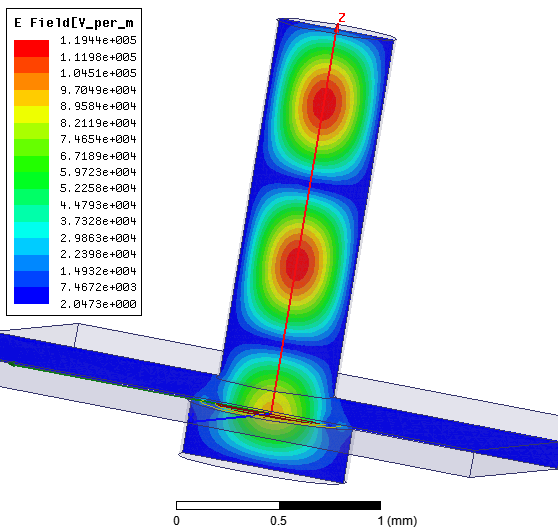
\includegraphics[width=3in]{images/ch4-hfss-model.png}
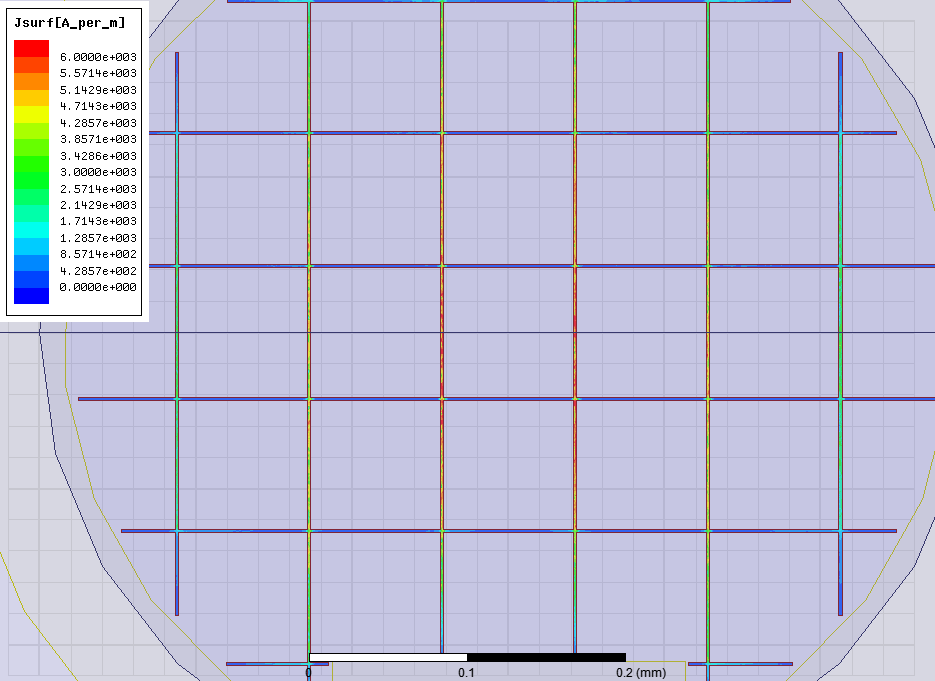
\includegraphics[width=3in]{images/ch4-hfss-grid.png}
\caption[\HFSS\ model]{
  Screen-shots taken from the \HFSS\ model used to simulate the absorbing grid.
  \textbf{Left}
  View of the full model, with the magnitude of the electric field plotted on a plane bisecting the model.
  \textbf{Right}
  Close-up view of the absorbing grid, with the surface current density plotted.
  The waveguide mode being excited is polarized in the up/down direction.
  Because the wires are thin compared to the width of the waveguide (\SI{2}{\um} vs \SI{600}{\um}), the current distribution is difficult to see in this plot.
  But close examination shows that the wires perpendicular to the excited polarization have very low current, while those parallel have higher current.
  The current decays towards the edges of the waveguide as expected.
}
\label{fig:ch4-hfss-model}
\end{figure*}

The results of these simulations are shown in \figref{fig:ch4-coupling}.
The band-averaged coupling efficiency of the mesh for unpolarized light is \SI{87}{\percent}.
Although the two polarizations have different absorption curves, with peak absorption at different frequencies, after averaging over the band their difference in efficiency is only \abt{\SI{1}{\percent}}.

Also shown in \figref{fig:ch4-coupling} is the frequency at which the TM01 waveguide mode turns on: \SI{383}{\GHz}.
Only \SI{0.9}{\percent} of the optical bandwidth is located above this frequency, so I have ignored any coupling to TM01 and all higher order modes.

\begin{figure*}
\centering
\includegraphics{./drawings/ch4-coupling.pdf}
\caption[Detector coupling efficiency]{
  Plot showing coupling efficiency of the detectors.
  The blue line is the transmission of the bandpass filter.
  The red and brown lines show the fractional power absorbed in the grid absorber.
  Although theses curves have different shapes, their integrated absorption over the band is within \SI{1}{\percent} of each other.
  The band-averaged absorption for unpolarized light is \SI{87}{\percent}.
  The blue dashed vertical line at \SI{383}{\GHz} indicates the cutoff frequency of the next-highest-order mode, TM01; \SI{0.9}{\percent} of the bandwidth is above this frequency.
}
\label{fig:ch4-coupling}
\end{figure*}

\figref{fig:ch4-coupling-mis} shows the effect of misalignment between the feedhorns and the detectors.
For small misalignment (less than $\SI{100}{\um} \approx \SI{4}{\mils}$) the loss in coupling efficiency is small.
But for large misalignment the loss is efficiency will be large, and one mode will couple much worse than the other.
Because the beam for each individual mode is elliptical, this differential mode-coupling will lead to elliptical beams.
This could be part of the explanation for the combination of poor optical efficiency and elliptical beams described in \chapterref{c:imaging}.

\begin{figure*}
\centering
\includegraphics{./drawings/ch4-coupling-mis.pdf}
\caption[Feedhorn / detector misalignment]{
  Plots showing impact of misalignment between feedhorns and detectors.
  The left plot shows band-averaged coupling efficiency vs misalignment, for misalignment in both $x$ and $y$ directions.
  The right plot shows the ratio of band-averaged coupling efficiency of the $x$-polarized mode to the $y$-polarized mode, again for misalignment in both $x$ and $y$ directions.
  For misalignment up to \SI{100}{\um} loss in coupling efficiency is small.
  But for large misalignment the efficiency drops substantially, and the modes couple very differently, which will lead to an elliptical beam.
}
\label{fig:ch4-coupling-mis}
\end{figure*}

A final important parameter of the feedhorn is its phase center, defined as the point along the axis of the horn from which the far-field spherical wavefront appears to emerge.
In order to achieve optimum performance from a system, the focal plane of the optical system should coincide with the phase centers of the horns.
The phase center of a conical feedhorn can not be defined in general, because it changes not only with polarization but with the beam angle as well.
For the \Imager\ I used published tables to estimate the location of the phase center for our feedhorns, which give a distance of \SI{0.9}{\mm} behind the opening of the feedhorn as the phase center averaged over both polarizations \cite[Page~353]{thomas_a._milligan_modern_2005}.

\section{Predicted Optical Efficiency and Optical Loading on Detectors} \label{sec:ch4-opt-eff}

The waveguide behind the feedhorns in the \Imager\ causes the detectors to be sensitive to only the two degenerate TE11 waveguide modes over \SI{99}{\percent} of their bandwidth.
Because some of the light detected by the \Imager\ is reflected, we expect the light to be polarized to some extent.
But to simplify the analysis, I assume here that the light is unpolarized, so that the detectors are sensitive to two uncorrelated waveguide modes.

The optical power from a source of temperature $T$ in a single mode detected by a detector with efficiency $\eta(\nu)$ is given by \cite{zmuidzinas_thermal_2003}
\begin{equation} \label{eqn:ch4-power-per-mode}
  P_{opt}(T) = \int \eta(\nu) h \nu n(\nu,T) d \nu ,
\end{equation}
where $n$ is the photon occupation number given by the Bose-Einstein factor
\begin{equation} \label{eqn:ch4-photon-n}
  n(\nu,T) = \frac{1}{e^{\frac{h \nu}{k_B T}} -1}.
\end{equation}
For \SI{350}{\GHz} light emitted by a \SI{300}{\K} source, $n \approx 17$, so the Raleigh-Jeans limit $h \nu \ll k_B T$ holds, and \eqnref{eqn:ch4-power-per-mode} simplifies to
\begin{equation} \label{eqn:ch4-power-per-mode-rj}
  2 k_B T \int \eta(\nu) d \nu = 2 k_B T \eta_{tot} \Delta \nu,
\end{equation}
where $\eta_{tot}$ is the total optical efficiency of the system and $\Delta \nu$ is the optical bandwidth.
My calculations below assume the exact from of \eqnref{eqn:ch4-power-per-mode}, but \eqnref{eqn:ch4-power-per-mode-rj} is useful for quick calculations and checks.

Photon \NEP\ is given by \cite[Equation~51]{zmuidzinas_thermal_2003}
\begin{equation} \label{eqn:ch4-photon-nep}
  \NEPph^2 = 4 \int (h \nu)^2 \eta(\nu) n(\nu,T) (1 + \eta(\nu) n(\nu,T)) d \nu.
\end{equation}
Here the second term represents ``photon bunching'', which only becomes important when many photons are occupying a spatial mode.
For millimeter and submillimeter astronomy observing cold sources such as the Cosmic Microwave Background Radiation, this second term is often negligible, but it is important for the \Imager\ because we are observing \abt{\SI{300}{\K}} targets.

There are two points worth noting about \eqnref{eqn:ch4-photon-nep}.
First, it is tempting to simplify \eqnref{eqn:ch4-photon-nep} as:
\begin{equation}
  \NEPph^2 = 4 (h \nu_0)^2 \eta_{tot} n(\nu_0,T) (1 + \eta_{tot} n(\nu_0,T)) \Delta \nu,
\end{equation}
where $\nu_0$ is the central frequency of the band.
However, this is not correct unless $\eta_{tot}$ and $\Delta \nu$ have been defined so that $\eta_{tot} = \int \eta^2(\nu) d\nu / \int \eta(\nu) d\nu$ and $\Delta \nu = \int \eta(\nu) d \nu / \eta_{tot}$.
I have not defined the bandwidth of the \Imager\ in this way, so I always evaluate the integral in \eqnref{eqn:ch4-photon-nep}.

Second, the \Imager\ is not viewing a single temperature $T$ that reaches the detectors with efficiency $\eta$.
Rather, the \Imager\ is viewing an \abt{\SI{300}{\K}} source that is attenuated by a series of lossy elements, each of which is at non-zero temperature and so emits power itself.
Because of the photon bunching term, it is not correct to calculate \NEPph\ for each optical component separately and then sum all values; doing so will underestimate the noise due to photon bunching.

The correct generalizations of \eqnref{eqn:ch4-power-per-mode} and \eqnref{eqn:ch4-photon-nep} are to treat the term $\eta(\nu) n(\nu,T)$ as an total photon occupation number that includes contributions from all sources.
I make the simplifying approximation that the frequency-dependence of the efficiency $\eta{\nu}$ is the same for all source of optical power; i.e., it is set by the bandpass filter alone.
The total occupation number absorbed in the detectors is then given by
\begin{equation} \label{eqn:ch4-tot-n0}
  \eta(\nu) n(\nu,T) \equiv \tau_{bp}(\nu) \sum_k \eta_k \epsilon_k n_k(\nu,T_k).
\end{equation}
Here $\tau_{bp}(\nu)$ is the transmission of the bandpass, $\eta_k = \prod_{k^{\prime} \le k} \epsilon_{k^{\prime}}$ is the cumulative efficiency for light from source $k$ to be absorbed in the detector, $\epsilon_k$ is the emissivity of source $k$ and $n(\nu,T_k)$ is the Bose-Einstein factor \eqnref{eqn:ch4-photon-n} for source $k$, which is at temperature $T_k$.

Under these assumptions the expression for optical power becomes
\begin{equation} \label{eqn:ch4-opt-pow-all}
  2 \int h \nu \tau_{bp}(\nu) \left( \sum_k \eta_k \epsilon_k n(\nu,T_k) \right) d \nu.
\end{equation}
Note that in this case the optical powers from each source can be calculated separately and then summed.
\NEPph\ is given by
\begin{equation} \label{eqn:ch4-nep-all}
  \NEPph^2 = 4 \int (h \nu)^2 \tau_{bp}(\nu) \left( \sum_k \eta_k \epsilon_k n(\nu,T_k) \right) 
       \left( 1 + \tau_{bp}(\nu) \left( \sum_k \eta_k \epsilon_k n(\nu,T_k) \right)  \right) d \nu.
\end{equation}

% \tableref{tab:ch4-opt-eff} lists all components of the \Imager\ and their contribution to optical efficiency.
\tableref{tab:ch4-opt-load} lists all components of the \Imager\ that contribute to optical loading.
For each component \eqnref{eqn:ch4-opt-pow-all} is integrated over the \Imager's optical band.
The temperatures listed for the filters inside the cryostat are estimates based on measurements described in \tableref{tab:ch4-filter-stack}.
Also listed are the photon occupation quantities $\epsilon_k \eta_k n(\nu_0,T_k)$ at the band-center frequency of $\nu_0 = \SI{347}{\GHz}$.
The predicted total optical loading on each detector is \SI{180}{\pW}, and the predicted optical $NEP_{ph} = \Pnoisef{0.85}$.

\begin{table*}
\centering
\caption[Optical load and photon noise]{
  Optical load and photon noise from all components in the \Imager.
  $P_{opt}$ for each component is calculated according to \eqnref{eqn:ch4-opt-pow-all}.
  $\epsilon \eta n$ is calculated at the center frequency of the band (\SI{347}{\GHz}) and also includes the transmission of the bandpass filter at that frequency.
  All powers are the power absorbed in the bolometer, and the \NEPph\ value is referred to power absorbed in the bolometer.
  The efficiency of the lens accounts for losses due to both reflection from the lens and absorption in the lens.
  ``Beam'' refers to power from the far-field that reaches detectors, while ``Spillover'' refers to power that reaches the detectors due to the portion of the beam that misses the primary mirror.
}
\label{tab:ch4-opt-load}
\begin{tabular}{ccccccc}
% The content of this table is producted by thesis/calc_optical_loading()
\toprule 
  Component  & 
  \specialcell{Temperature \\ (\si{\K})} & 
  Efficiency & 
  Emissivity & 
  \specialcell{$P_{opt}$ \\ (\si{\pW})} & 
  $\epsilon \eta n$ & 
  \specialcell{Cumulative \\ Efficiency} \\  
\midrule 
  Bolometer  &   1 & 0.87 &      &       &      & 0.87 \\ 
  Feedhorn   &   1 & 0.91 &      &       &      & 0.79 \\ 
  W1275      &   5 & 0.89 &      &       &      & 0.70 \\ 
  W1266      &  16 & 0.98 & 0.02 &   0.1 &  0.0 & 0.69 \\ 
  W1269      &  85 & 0.94 & 0.06 &   2.9 &  0.2 & 0.65 \\ 
  W1428      & 200 & 0.96 & 0.04 &   4.7 &  0.3 & 0.62 \\ 
  Lens       & 295 & 0.84 & 0.16 &  27.7 &  1.5 & 0.52 \\ 
  Beam       & 295 & 0.52 & 0.48 &  69.5 &  3.8 & 0.27 \\ 
  Spillover  & 295 & 0.00 & 1.00 &  75.3 &  4.1 & 0.00 \\ 
\midrule 
  Total      &     &      &      & 180.2 &  9.8 & 0.27 \\ 
\midrule 
  Total \NEPph\ & \Pnoise{0.85e-15} &   &  & & & \\ 
\bottomrule
\end{tabular}
\end{table*}

\section{Detector Readout} \label{sec:det-readout}

As described in \chapterref{c:tes}, the \Imager's detectors are voltage-biased, so that the detector output signal is a changing current.
To read out the detectors a low-noise current amplifier is required.
The \Imager\ uses a multiplexed \SQUID\ readout system to accomplish this.

A \SQUID\ is a Superconducting Quantum Interference Device \cite{clarke_squid_2002}.
For the purposes of understanding the operation of the \Imager, it suffices to know that a \SQUID\ is a very sensitive magnetometer, and by coupling the magnetic field produced by a current into the \SQUID, the \SQUID\ can also be used to read out a current signal.

An important aspect of the response of a \SQUID\ to an input current is that the response is not linear; it is periodic.
\figref{fig:tes-bias-ramp-sc} and \figref{fig:tes-bias-ramp-trans} show examples of this behavior for the \SQUIDs\ used in the \Imager.
This periodic response means that the readout system is not measuring the absolute current passing through the detectors, but rather changes in the current from some offset value, an offset value which is not known and can be different for each detector.
When processing a set of detector outputs into a video, these detector offsets must be accounted for.
The algorithm used to do this is described in \sectionref{sec:ch7-algo}.

To reduce the number of wires running into the cryostat, the \Imager\ uses a time-division multiplexed (\TDM) readout system \cite{chervenak_superconducting_1999,korte_time-division_2003,reintsema_prototype_2003}.
\figref{fig:ch4-tdm-schematic} shows a schematic of this readout system.
The detectors are divided into a columns, each column containing 32 rows.
Each detector output is coupled into the input coil of its own ``1st-stage'' \SQUID.
Row address lines bias the 32 rows sequentially, so that at any given time only one detector per column is being read out by the system.
This sequential addressing means that the current noise power spectral density of the \SQUIDs\ is increased by a factor of 32 due to aliasing, but the current noise in the \Imager's \SQUIDs\ is low enough that \SQUID\ noise is not a significant contribution to the total noise of the detectors.
See, e.g., \figref{fig:rsh-l-plots} and \figref{fig:ch6-trans-noise} for a demonstration that \SQUID\ noise (\abt{\Inoise{1e-10}}) is below the typical noise level of a detector biased into its standard operation conditions (\abt{\Inoise{1e-9}}).
To linearize the \SQUID\ amplifier chain, feedback in the form of magnetic flux is applied to the 1st-stage \SQUIDs.

\begin{figure*}
\centering
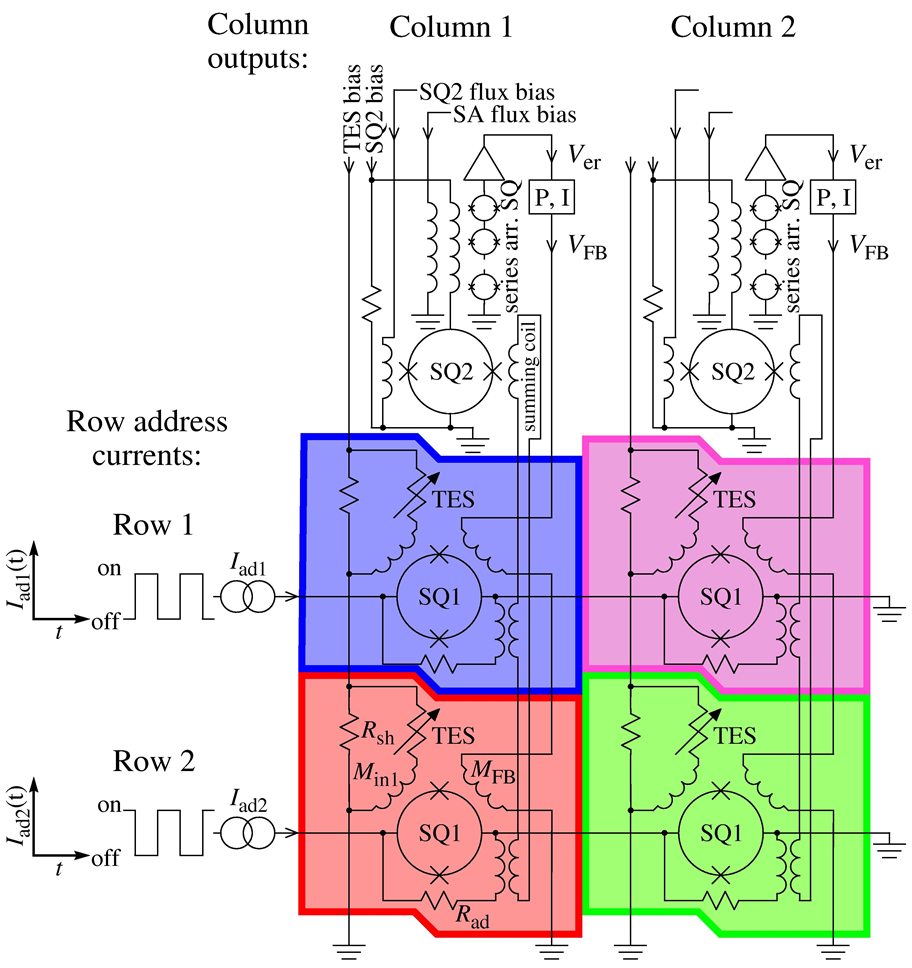
\includegraphics[width=3in]{images/ch4-tdm-schematic.png}
\caption[Time-Division Multiplexing Schematic]{
  Schematic of the Time-Division Multiplexing (\TDM) readout system used by the \Imager.
  The detectors are divided into rows and columns (2 each shown here).
  Each detector is coupled to its own 1st-stage \SQUID (\SQ1).
  At any given time, only one row of \SQUIDs\ is biased, indicated via the ``Row address currents'' on the left.
}
\label{fig:ch4-tdm-schematic}
\end{figure*}

A set of electronics is required to control the multiplexed readout system and provide data to a computer for further analysis.
The \Imager\ uses the Multi-Channel Electronics (\MCE) as the electronics control system \cite{battistelli_functional_2008,battistelli_automated_2008,_mcewiki_2014}.
The \MCE\ was developed in order to allow simple, remote operation of \TDM\ readout systems for submillimeter and millimeter astronomy.
It comes equipped with a software suite for controlling the electronics itself.
The entire electronics system for reading out 1024 detectors is contained within a single $\SI{15}{\in} \times \SI{14}{\in} \times \SI{14}{\in}$ crate drawing \SI{175}{\W}.
All communication with the controlling data acquisition computer is via a pair of fiber optic cables.
See \figref{fig:ch4-mce-photo} for a photo of the \MCE.

\begin{figure*}
\centering
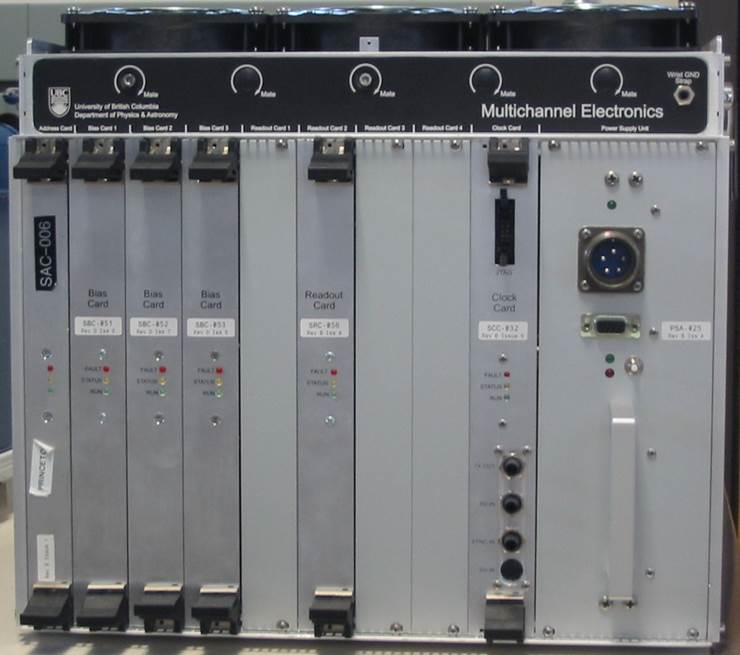
\includegraphics[width=3in]{images/ch4-mce.jpg}
\caption[Photograph of the \MCE]{
  Photograph of the \MCE\ unit used to readout the \Imager's detectors.
  The \MCE\ is \SI{15}{\in} wide.
}
\label{fig:ch4-mce-photo}
\end{figure*}

The \MCE\ has many parameters that can be set to control its behavior, almost none of which I will describe here.
The exceptions are the parameters that control the readout rate of the system, listed in \tableref{tab:ch4-mce-parms}.
The table also gives the value of these parameters used by the \Imager\ when taking videos.
The rate at which data is reported to the data acquisition computer is given by
\begin{equation} \label{eqn:ch4-mce-readout-rate}
  f_{ro} = \frac{ \SI{50}{\MHz} }{\texttt{row\_len} \times \texttt{num\_rows} \times \texttt{data\_rate} }
\end{equation}
Using the values in \tableref{tab:ch4-mce-parms} the readout rate is \SI{3125}{\Hz}.

Using any value for \texttt{data\_rate} other than 1 will lead to aliasing of noise.
As discussed in \sectionref{sec:ch6-aliasing}, this raises the total amount of noise in the \Imager's detectors by \SI{14}{\percent} on average.
This noise aliasing penalty can be reduced by configuring the \MCE\ to internally apply a digital 4-pole lowpass filter prior to reporting data to the data acquisition computer \cite{mce_team_digital_????}.

\begin{table*}
\centering
\caption[Configuration parameters for the \MCE]{
  A few important configuration parameters for the \MCE.
}
\label{tab:ch4-mce-parms}
\begin{tabular}{lcp{4in}}
% The content of this table is producted by thesis/calc_optical_loading()
\toprule 
  Parameter  & 
  Typical Value & 
  Explanation \\  
\midrule 
  \texttt{row\_len}  & 100 &
           Number of \SI{50}{\MHz} clock cycles spent on each row.  \\
  \texttt{num\_rows} & 32 &
           Number of rows to cycle over. \\
  \texttt{data\_rate} & 5 & The \MCE\ only reports every \texttt{data\_rate}-th sample to the data acquisition computer. \\
\bottomrule
\end{tabular}
\end{table*}
\section{Acknowledgments}

Bob Schwall of \NIST\ designed the cryostat, assembled the \He4-sorption fridge, and provided useful advice and help in the lab during commissioning of the cryostat.
Bob Schwall and William Duncan of \NIST\ designed the cryostat/mirror mount and the \He4 sorption refrigerator.
The refrigerator was filled with \He4 by Simon Dicker at the University of Pennsylvania.
Bob Schwall, Cale Gentry, and Ilya Smirnov wrote the LabVIEW program used to control the cryogenic system.
William Duncan designed, procured, and assembled the optical system.
The optical filters were designed by Peter Ade's group at Cardiff University in collaboration with William Duncan, and manufactured and measured at Cardiff.
The \MCE\ was provided by Mark Halpern's group at the University of British Columbia.
Mandana Amiri and Matthew Hasselfield provided extensive, timely and invaluable support for the \MCE\ hardware and software.
Cale Gentry provided much help in the lab while taking initial still images with prototype detectors.

